%%%
%%% Talk for Open Day 2022
%%% Updated jobs titles (where available) 200619
%%%
%%%
\documentclass{beamer}
\usepackage{graphics}
\usepackage{amsfonts}
\usepackage{colortbl}
\usepackage{multimedia}
\graphicspath{{pictures/}}
\graphicspath{{../pictures/}}
\usetheme{default}%Singapore}
\definecolor{paleblue}{rgb}{.75,0.75,1}
\definecolor{darkgreen}{rgb}{.2,.8,0}
\definecolor{pink}{rgb}{1,.5,0.75}

\newcommand{\blue}{\color{blue}}
\newcommand{\red}{\color{red}}
\newcommand{\black}{\color{black}}
\newcommand{\itema}[1]{\item<#1-| alert@#1>}
\newcommand{\on}[1]{\onslide<#1->}

\graphicspath{{pictures/}}

\title{Opening Doors\\
 Mathematics Careers and Degrees}
%\author{Dr Matthew Craven\\matthew.craven@plymouth.ac.uk\\Centre for Mathematical Sciences}
%%\author{Dr Gosia Wojtys\\malgorzata.wojtys@plymouth.ac.uk\\Centre
%%for Mathematical Sciences}

\author{Dr Craig McNeile\\craig.mcneile@plymouth.ac.uk\\Centre for Mathematical Sciences}

\date{}

\begin{document}
\frame{\titlepage

\begin{center}
\includegraphics[height=1.6cm]{UoP_Logo_Centred_Colour.jpg}
\end{center}
%\vspace{-1.2cm}
%\blue \rightline{\bf 4th in the Guardian Mathematics}
%\rightline{\bf University League Table 2020\black}

}


\section{Introduction}

\subsection*{MS}


\section*{Surprises}

\subsection*{surprises}

\frame{\frametitle{The Many Branches of Mathematics}

\bigskip

\begin{tabular}{cc}
  % after \\: \hline or \cline{col1-col2} \cline{col3-col4} ...
  \begin{minipage}{.3\linewidth}
\begin{center}
\includegraphics<2>[width=3cm]{mahle.png}
%%\includegraphics<3>[width=3cm]{tsp.png}
\includegraphics<3>[width=3cm]{Petersen-graph.png}
%\includegraphics<4>[width=3cm]{tiling.png}
\includegraphics<4>[width=5cm]{football-fig3.png}
\includegraphics<5>[width=4cm]{simul8.png}
%%\includegraphics<5>[width=3cm]{Petersen-graph.png}
\includegraphics<6>[height=3cm,width=4cm,angle=270,origin=c]{martins-phone.jpg}
%%\includegraphics<7>[width=3cm]{Plymouth_GPU.jpg}
\includegraphics<7>[width=4cm]{small_HPC_image.png}
\includegraphics<8>[width=3cm]{ValerieMillar2.jpg}
\end{center}
{}\null
 \end{minipage}
&  
\begin{minipage}{.7\linewidth}
\begin{itemize}
\item<2-| alert@2> Applied Mathematics:\\ calculus is its language; fluids to finance
\item<3-| alert@3> Pure mathematics:\\
underlying structures and symmetries
\item<4-| alert@4> Probability and statistics:\\ calculus and computing ($\mathsf{\textbf{R}}$)
\item<5-| alert@5> Operational research:\\
  logistics, planning, simulations, optimisation
  \item<6-| alert@6> Theoretical physics:\\
  quantum theory, relativity
  \item<7-| alert@7> Programming:\\
  Python, $\mathsf{\textbf{R}}$, Excel, supercomputing (HPC), GPU teaching/research centres
    \item<8-| alert@8> Communication skills!
\end{itemize}
 \end{minipage}
\end{tabular}

}

\frame{\frametitle{Mathematics Makes You Very Employable}%

Professional experience is so important \dots\ but so is mathematics

%%\on2
\begin{center}
\[
\begin{array}{cc}
\hspace{-.4cm}\begin{minipage}[c]{7.9cm}
{\blue \it \lq\lq  When I left Cond\'e Nast, they advertised for a new intern and changed the job description to ask candidates to have a maths/statistics based degree with a good understanding of Excel. This was changed after I had worked with them and they then realised how much a maths graduate could bring to the company.\rq\rq}\\
\rightline{Rebecca Ruane}
\rightline{Analytics Manager}
\rightline{Guardian News \& Media}
\end{minipage}
&
\begin{minipage}[c]{3cm}
\begin{center}\includegraphics[width=3cm]{RebeccaWhawell}\\[5mm]
\end{center}
\null
\end{minipage}
\end{array}
\]
(A demonstrable impact on intern recruitment.)
\end{center}
}

\section*{Good Degrees to Study}
\subsection*{good degrees to study}

\frame{\frametitle{Contents?}

\[
\begin{array}{rr}
\begin{minipage}[r]{7cm}
\begin{itemize}
    \item First year partly what you expect (calculus, vectors, matrices).
    \item Much more rigour (proof).
%%    \item But many surprises \dots
    \item More choice in final year.
    \item Assessment: generally 60-80\% exam, plus coursework (CW). Some CW-only modules.
\end{itemize}
\end{minipage}
   & \begin{minipage}[l]{5cm}
\begin{center}
\includegraphics[width=4cm]{geometri.png}
\end{center}
\end{minipage} \\
\end{array}
\]

\medskip

\[
\begin{array}{rr}
\begin{minipage}[r]{2cm}
\begin{center}
\includegraphics[width=2cm]{Duane_Appleby2W}
\end{center}
\end{minipage}
   & \begin{minipage}[l]{8.2cm}
{\color{blue} \it \lq\lq My final year project on quantum computing helped me to show
my technical awareness and show that I was looking at some of the
leading research in computing at the time.\rq\rq} \\
{Duane Appleby, IT Specialist IBM} % Cannot find profile on linked in (as of 200619)
\end{minipage} \\
\end{array}
\]

}

\frame{\frametitle{Student Support}
\begin{center}
\includegraphics[width=6.2cm]{PALS.jpg}
\end{center}
\vspace{-1cm}
\begin{center}
\begin{minipage}[c]{14cm}
\begin{itemize}
    \item Support classes (tutorials, PALS)
    \item Personal tutor system
    \item Drop in centres
    \item Approachable lecturers
    \item 15 hours of classes (lectures, computer labs etc.) per week. 
    \item Employability sessions delivered by professional Careers Advisors
   % \item[] (The same amount of private study is required.)
\end{itemize}
\end{minipage}
\end{center}
}

\frame{\frametitle{Student Support}
\begin{center}
\includegraphics[width=5cm]{iPadmini.jpg}
\end{center}
\begin{center}
\begin{minipage}[c]{14cm}
Technology to help teaching and learning:
\begin{itemize}
  \item lecture notes
  \item lectures are recorded
  \item podcasts (by staff and students)
  \item voting/instant feedback
\end{itemize}
\end{minipage}
\end{center}

}



\frame{ \frametitle{A Track Record of Satisfied Students}

\begin{center}

\includegraphics[scale=0.1]{TEF_Gold2.jpg}
\end{center}
\vspace{-8mm}

\[
\hspace{-8mm}
\begin{array}{rr}

\begin{minipage}[r]{7.8cm}
{\textbf{\noindent
Consistent high scores for students' satisfaction.}}
\vspace{3mm}
Guardian Mathematics League Table

\begin{itemize}
\item  2023: {\red \textbf{2$^{\textrm{nd}}$}} satisfaction with Mathematics teaching.

\item  2022: {\red \textbf{6$^{\textrm{th}}$}} satisfaction with Mathematics teaching.

%%\begin{itemize}
%    \item {\red \textbf{6$^{\textrm{th}}$}} in the UK for satisfaction with Mathematics teaching.
%%    \item {\red \textbf{2$^{\textrm{nd}}$}} in the UK for Value added score.\vspace{3mm}\\
%\end{itemize}


\item 2021: {\red \textbf{8$^{\textrm{th}}$}} satisfaction with
  Mathematics teaching.
  %%\vspace{3mm}\\


\item 2020: {\red \textbf{4$^{\textrm{th}}$}} overall in the UK.
  %% \vspace{3mm}\\


%%\item 2019: {\red \textbf{Top}} of the UK for satisfaction with the course.
%\item {\red \textbf{4$^{\textrm{th}}$}} in the UK for satisfaction with Mathematics teaching.


%2018 National Student Survey
%
%\begin{itemize}
%\item {\red \textbf{99\%\  }} Staff are good at explaining things.
%\item {\red \textbf{99\%\  }} I have had the right opportunities to work with other students as part of my course.
%\end{itemize}

\end{itemize}

{\red  85 \%} of mathematics graduates,
from this school, were working in a graduate jobs after 15 months
(Guardian league table 2023)

\end{minipage}

& 
\begin{minipage}[l]{4.5cm}
\begin{center}
\hspace{-3mm}\includegraphics[width=4.5cm]{clickerscropped.jpg}
\end{center}
\end{minipage} 

\end{array}
\]
}


\frame{ \frametitle{Placements and Careers}
\[
\begin{array}{rr}
\begin{minipage}[r]{7cm}
Year long placements (typically earn \pounds 20\,k)
%  2023 updated placement to 20K 
\vspace{-0.3cm}
\begin{itemize}
    \item Employers include:
    \begin{itemize}
      \item Mastercard
      \item Glaxo-Smith-Kline, Eli Lilly\dots
      \item ONS, DSTL
    \end{itemize}
    \item Very successful on return
\end{itemize}
Other placements
\begin{itemize}
\item Summer placements in industry.
\item Our School runs a summer internship scheme for undergraduate
      research projects (\pounds 2\,k)
    \item School placement module
\end{itemize}
Careers fairs
\begin{itemize}
    \item Events and talks 
    \item E.g., our own Maths Careers conference
\end{itemize}
\end{minipage}
   & \begin{minipage}[l]{4.5cm}
\begin{center}
\hspace{-3mm}\includegraphics[width=4cm]{placements2.jpg}
\end{center}
\end{minipage} \\
\end{array}
\]
}

%{
%\usebackgroundtemplate{\includegraphics[width=\paperwidth]{placements2016}}
%\begin{frame}[plain]
%\end{frame}
%}

\section*{Careers}
\subsection*{careers}


\frame{\frametitle{Which Careers are Open?}

\noindent
\onslide<1-2>Almost any!

\onslide<2->


\begin{tabular}{cl}
  % after \\: \hline or \cline{col1-col2} \cline{col3-col4} ...
  \begin{minipage}{.44\linewidth}
%\includegraphics<2>[width=4cm]{GaryCottle.jpg}
\includegraphics<2>[width=4cm]{rdodge.jpg}
\includegraphics<3>[width=4cm]{george.jpg}
\includegraphics<4>[width=4cm]{Lizzy.jpg}
%\includegraphics<5>[width=5cm]{JamiePartridge}
\includegraphics<5>[width=4.5cm]{DanPalomeque.jpg}
%\includegraphics<7>[width=4.5cm]{DavidJonescropped.jpg}
  \end{minipage} &
  \begin{minipage}{.56\linewidth}
\begin{itemize}
 \item<2-| alert@2>Rebecca Dodge: \pounds 25k IMA Teaching Scholarship \\\vspace{3mm} % Checked 200619
  \item<3-| alert@3> George Nemeshanyi: Software Engineer, EFFECT Photonics \\\vspace{3mm} % Updated Sept-2022
  \item<4-| alert@4> Lizzy Goult: Doctoral Researcher, Max Planck Institute for Infection Biology \\\vspace{3mm} % Updated Sept-2022
  %\item<5-| alert@5> Jamie Partridge: Research, Cambridge \\ % Could not find 200619
 \item<5-| alert@5> Daniel Palomeque: Senior Actuarial Analyst, Zurich Australia \\\vspace{3mm} % Checked Sept-2022
 %\item<7-| alert@7>.David Jones: Sports Trader, Betvictor % Could not find (200619)
  \end{itemize}
   \end{minipage}
\end{tabular}
}



\frame{\frametitle{Medical Research and Development}%

\begin{center}

Evidence-based medicine requires statistics
\end{center}



\bigskip
\includegraphics[width=3.5cm]{Jennifer_Lannon.jpg}%lindsay_thompson.jpg}
\includegraphics[width=3.5cm]{shaunbedford}
\includegraphics[width=3.5cm]{milensu.jpg}

\begin{center}\hspace{-4mm}
\begin{minipage}{.33\linewidth}
\begin{center} {\it Jenny Lannon}\\ % Cannot find on LinkedIn (as of 200619)
Principal Statistician\\
NHS Blood and Transplant
\end{center}
\end{minipage}
\begin{minipage}{.33\linewidth}
\begin{center}{\it Shaun Bedford}\\
Associate Global Trial Director\\
Novartis, IQVIA % as of 200619
\end{center}
\end{minipage}
\begin{minipage}{.33\linewidth}
\begin{center}{\it Milensu Shanyinde}\\ % Checked on 200619
PhD at UCL\\
Senior Medical Statistician\\ at CTU Oxford
\end{center}
\end{minipage}
\end{center}
}


\frame{\frametitle{The Financial World}

\vspace{-5mm}

\begin{center}
\[
\hspace{-1cm}\begin{array}{cc}
\begin{minipage}[c]{3cm}
\begin{center}\includegraphics[width=3cm]{dom}\\[5mm]
\end{center}
\null
\end{minipage}
   &
\begin{minipage}[c]{8cm}
{\blue \it \lq\lq The most useful aspect of a Mathematics degree is the problem solving skills you acquire.\rq\rq}\\
\rightline{Dominic Klee} % Checked 200619 (manager -> senior manager)
\rightline{Senior Portfolio Manager}
\rightline{State Street Global Advisors}
\end{minipage}
\end{array}
\]
\end{center}

\on2

\begin{center}
\[
\hspace{-1cm}\begin{array}{cc}
\begin{minipage}[c]{8cm}
Chartered accountant, winner of International\\ Order of Merit for Financial Accounting\\
\rightline{Charlotte Wells} % Could not find on LinkedIn (as of 200619)
\rightline{Manager, Francis Clark LLP}
\end{minipage}
   &\begin{minipage}[c]{3cm}
\begin{center}
\includegraphics[width=3cm]{CharlotteWells}\\[5mm]
\end{center}
\null
\end{minipage}
\end{array}
\]
\end{center}

}

\frame{\frametitle{Industry and Engineering}

\vspace{-1cm}
\begin{center}
\[
\begin{array}{cl}
\begin{minipage}[c]{7cm}
Tomasz Szyrowski\\{\color{blue} PhD in Marine Engineering}{\color{red}
\begin{itemize}
        \item Mathematical modelling of how to detect undersea cables
    \item Brand new approach\\ (using Monte Carlo techniques)
    \item Scientific Software Developer at the Met Office % Updated 200619
    \item Lead Software Engineer at HMRC
    \end{itemize}}
\end{minipage}
   &
   \begin{minipage}[c]{3cm}
\begin{center}
\vspace{7mm}\onslide<1->\includegraphics[width=4cm]{TSzyrowski_boat1.jpg}\\
\end{center}
\null
\end{minipage}
\end{array}
\]
\end{center}
}


\frame{\frametitle{Computing}

%\begin{center}
%{\it Trust the math. Encryption is your friend. Use it well, and do your best to ensure that nothing can compromise it. }
%\end{center}
%{\small Bruce Schneier (Cryptographer and Privacy Activist), Harvard Law School} % Checked 200619
%
%\bigskip\medskip
%
%\onslide<2->

\begin{tabular}{cc}
  \begin{minipage}{.35\linewidth}
\begin{center}

\includegraphics[width=3.5cm]{computing2.png} 
\end{center}
{}\null
 \end{minipage}
&  

\begin{minipage}{.5\linewidth}Peter von Holy\\
Bioinformatics Scientist, GSK\\% Checked Sept-2022

{\blue \it \lq\lq \small
Programming is logic-based. \\

While on my placement in BAE, I was commended for my fast learning capabilities, as I became proficient in JavaScript over the course of the placement, as well as my ability to solve complex problems.\\

Then, I was able to demonstrate my skills in a coding challenge given to me during the application process in GSK.\rq\rq}
 \end{minipage}
\end{tabular}

}

\frame{\frametitle{Climate}

\begin{center}
\includegraphics[width=4cm]{peter_jermey}
%\href{run:CNasir.wmv}{\includegraphics[width=4cm]{claire.jpg}}
\end{center}


\bigskip\noindent
{\color{blue}\it \lq\lq My degree gave me an essential introduction to numerical mathematics and mathematical programming which are the basis of modern applied mathematics in all industries.\rq\rq}
\\
Peter Jermey, {\bf Met Office} % Could not find 200619

}

%%
\frame{\frametitle{Final year projects}

  There is a lot of academic content in the degree. For example,
  below are a few titles of final year projects.

  \begin{itemize}

%\item Smooth Manifolds and Riemannian Geometry.
\item Learning Phases of Matter with Neural Networks.
\item Algebraic solutions of the hypergeometric equation.
\item Elliptic Curve Cryptography: A Mathematical Arms Race.
\item Differential geometry and Einstein’s Field Equations.
\item Using Machine Learning to Diagnose Pneumonia from Covid-19 in Patients from
Chest X-Rays
  
\end{itemize}
    
%%  src = https://en.wikipedia.org/wiki/Isaac_Newton
\begin{center}
  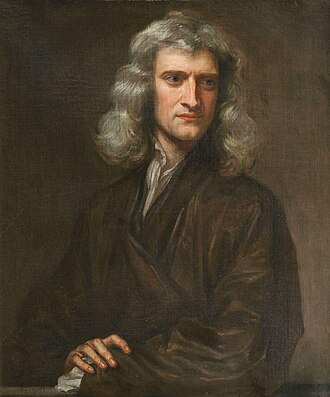
\includegraphics[scale=0.2]{Portrait_of_Sir_Isaac_Newton.jpg}
\end{center}
After inventing calculus, mechanics and gravitation, Sir Isaac Newton
became the warden of the Royal Mint.

}

\section{Conclusion}
\subsection*{concl}

\frame{\frametitle{Summary}

\noindent Mathematics is beautiful and helps you understand the world around you.
But it also opens doors to exciting and well paid careers:

\begin{center}
\[
\begin{array}{cc}
\begin{minipage}[c]{7cm}
{\color{red} \null\begin{itemize}\vspace{-16mm}
\item {\color{black} Mathematics degrees keep more options open}\vspace{3mm}
\item {\color{black} Lots of support during your studies\\ \href{http://www.youtube.com/watch?v=nwvJWYqMoyk}{(modern technology)}}\vspace{3mm}
\item {\color{black} Students enjoy our degrees (NSS, Guardian)}\vspace{3mm}
\item {\color{black} They lead to well paid and extremely interesting jobs}%\onslide<2->
    \end{itemize}}
\end{minipage}
   &
   \begin{minipage}[c]{4cm}
\begin{center}\onslide<1->
\includegraphics[width=3.4cm]{girl_lib.jpg}
\end{center}
\null
\end{minipage}
\end{array}
\]
\end{center}


}



%\frame{\frametitle{Rest of Today?}

%\noindent The University is offering many activities and people to speak to.

%\bigskip\medskip

%\noindent In Mathematics:\vspace{-8mm}
%\begin{center}
%\[
%\begin{array}{cc}
%   \begin{minipage}[c]{4cm}
%\begin{center}
%\includegraphics[width=3.4cm]{bubbles3.jpg}
%\end{center}
%\null
%\end{minipage}
%   &
%\begin{minipage}[c]{7cm}
%{\color{red} \null\begin{itemize}\vspace{-16mm}
%\item {\color{black} A drop in session until %4\,pm\\ This room.}
%\item {\color{blue} A talk on the content of our %Mathematics degrees\\ This room at 1 pm (Dr Anton %Ilderton)}
%\item {\color{red} Key opportunity: talk to staff %and current students}
%    \end{itemize}}
%\end{minipage}
%\end{array}
%\]
%\end{center}
%}

\end{document}
